\documentclass{beamer}
\title{Constructing Lagrangian torus fibrations}
\author{Jonny Evans}
\date{joint with Mirko Mauri}
\usenavigationsymbolstemplate{}
\usepackage[utf8]{inputenc}
\usepackage[T1]{fontenc}
\usepackage{fixltx2e}
\usepackage{graphicx}
\usepackage{longtable}
\usepackage{float}
\usepackage{parallel}
\usepackage{parcolumns}
\usepackage{wrapfig}
\usepackage{rotating}
\usepackage{amsmath}
\usepackage{textcomp}
\usepackage{marvosym}
\usepackage{wasysym}
\usepackage{amssymb}
\usepackage{amsthm,amsmath,amsfonts,amscd,setspace}
\renewcommand{\partname}{Week}
\usepackage{tikz}
\usetikzlibrary{decorations.markings,decorations.pathmorphing,shapes}
\usepackage{parskip}
\newcommand{\FF}{\mathfrak{f}}
\newcommand{\GG}{\mathfrak{g}}
\newcommand{\CC}{\mathbb{C}}
\newcommand{\QQ}{\mathbb{Q}}
\newcommand{\RR}{\mathbb{R}}
\newcommand{\UU}{\mathbb{U}}
\newcommand{\XX}{\mathbb{X}}
\newcommand{\YY}{\mathbb{Y}}
\newcommand{\ZZ}{\mathbb{Z}}
\newcommand{\Link}{\operatorname{Link}}
\newcommand{\Cone}{\operatorname{Cone}}
\newcommand{\colim}{\operatorname{colim}}
%\newcommand{\amal}{\operatorname{amal}}
\newcommand{\adj}{\operatorname{adj}}
\newcommand{\cp}[1]{\mathbf{CP}^{#1}}
\newcommand{\rp}[1]{\mathbf{RP}^{#1}}
\newcommand{\OP}[1]{\mathrm{#1}}
\newcommand{\ma}{\begin{pmatrix}}
\newcommand{\mz}{\end{pmatrix}}
\newcommand{\tka}{\begin{center}\begin{tikzpicture}}
\newcommand{\tkz}{\end{tikzpicture}\end{center}}
\newcommand{\matr}[4]{\left(\begin{array}{cc}#1 & #2\\ #3 & #4\end{array}\right)}
\newcommand{\mthrthr}[9]{\left(\begin{array}{ccc}#1 & #2 & #3\\ #4 & #5 & #6\\ #7 & #8 & #9\end{array}\right)}
\newcommand{\vect}[2]{\left(\begin{array}{c}#1\\#2\end{array}\right)}
\newcommand{\vthr}[3]{\left(\begin{array}{c}#1\\#2\\#3\end{array}\right)}
\newcommand{\TO}[3]{#1\stackrel{#2}{\longrightarrow}#3}
\makeatletter
\renewcommand*\env@matrix[1][*\c@MaxMatrixCols c]{%
  \hskip -\arraycolsep
  \let\@ifnextchar\new@ifnextchar
  \array{#1}}
\makeatother

\begingroup
\makeatletter
\@for\theoremstyle:=definition,remark,plain\do{%
\expandafter\g@addto@macro\csname th@\theoremstyle\endcsname{%
\addtolength\thm@preskip\parskip
}%
}
\endgroup
\usepackage{graphicx}
\usepackage[capitalise]{cleveref}
%\newtheorem{Theorem}{Theorem}[section]
%\newtheorem{Lemma}[Theorem]{Lemma}
%\newtheorem{Corollary}[Theorem]{Corollary}
%\newtheorem{Proposition}[Theorem]{Proposition}
%\theoremstyle{remark}
%\newtheorem{Remark}[Theorem]{Remark}
%\theoremstyle{definition}
%\newtheorem{Definition}[Theorem]{Definition}
%\newtheorem{Example}[Theorem]{Example}
%\newtheorem{Exercise}[Theorem]{Exercise}
%\newtheorem{Question}[Theorem]{Question}
%\newtheorem{Solution}[Theorem]{Solution}
%\newtheorem{Answer}[Theorem]{Answer}
\crefname{Theorem}{Theorem}{Theorems}
\Crefname{Theorem}{Theorem}{Theorems}
\crefname{Lemma}{Lemma}{Lemmas}
\Crefname{Lemma}{Lemma}{Lemmas}
\crefname{Corollary}{Corollary}{Corollaries}
\Crefname{Corollary}{Corollary}{Corollaries}
\crefname{Claim}{Claim}{Claims}
\Crefname{Claim}{Claim}{Claims}
\crefname{Proposition}{Proposition}{Propositions}
\Crefname{Proposition}{Proposition}{Propositions}
\crefname{Remark}{Remark}{Remarks}
\Crefname{Remark}{Remark}{Remarks}
\crefname{Definition}{Definition}{Definitions}
\Crefname{Definition}{Definition}{Definitions}
\crefname{Example}{Example}{Examples}
\Crefname{Example}{Example}{Examples}
\crefname{Exercise}{Exercise}{Exercises}
\Crefname{Exercise}{Exercise}{Exercises}
\crefname{Question}{Question}{Questions}
\Crefname{Question}{Question}{Questions}
\crefname{Solution}{Solution}{Solutions}
\Crefname{Solution}{Solution}{Solutions}
\crefname{Answer}{Answer}{Answers}
\Crefname{Answer}{Answer}{Answers}
\crefformat{footnote}{#2\footnotemark[#1]#3}

\begin{document}
\maketitle
\begin{frame}
\begin{overprint}
\onslide<1>
\begin{Theorem}[Gross 1999]\label{thm:gross}
Many Calabi-Yau 3-folds admit topological torus
fibrations over \(S^3\) with singular fibres over a
trivalent graph.
\end{Theorem}
\onslide<2>
\begin{block}{Question}
\begin{itemize}
\item Can we make these fibrations Lagrangian?
\item Even just (semi-)locally?
\end{itemize}
\end{block}
\onslide<3>
\begin{block}{Positive vertex: Yes!}
\begin{align*}
F&\colon\CC^3\setminus\{xyz-1=0\}\to\RR^3\\
F(x,y,z)&=\left(|x|^2-|y|^2,|x|^2-|z|^2,|xyz-1|\right)
\end{align*}
\end{block}
\onslide<4>
\begin{block}{Negative vertex: ?}
\[F\colon\CC^3\setminus\{(xy-z-1)z=0\}\to\RR^3?\]
\end{block}
\onslide<5>
\begin{block}{Negative vertex: Yes!}
\[F\colon\CC^3\setminus\{(xy-z-1)z=0\}\to\RR^3\]
\end{block}


\end{overprint}
\begin{overprint}
\onslide<1-4>
\begin{center}
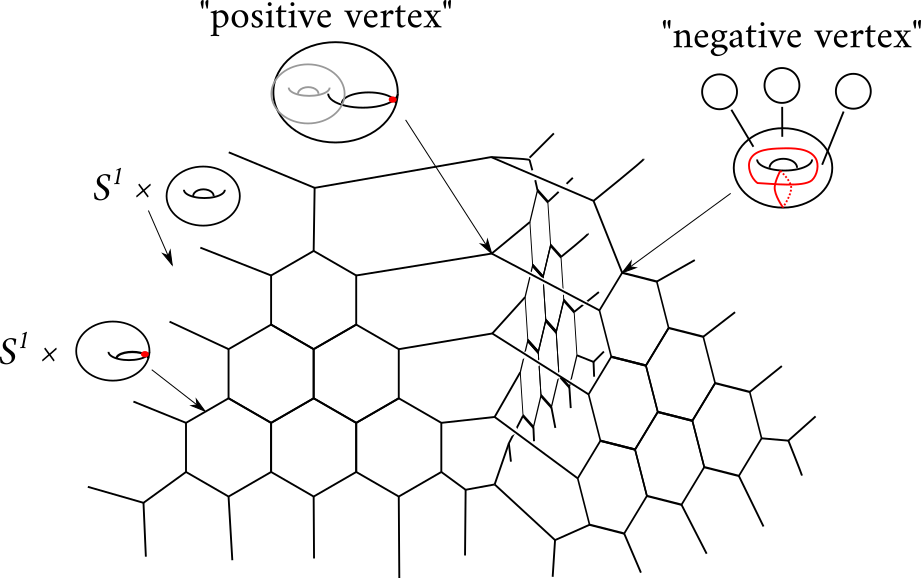
\includegraphics[width=250pt]{discriminant}
\end{center}
\onslide<5>
\begin{center}
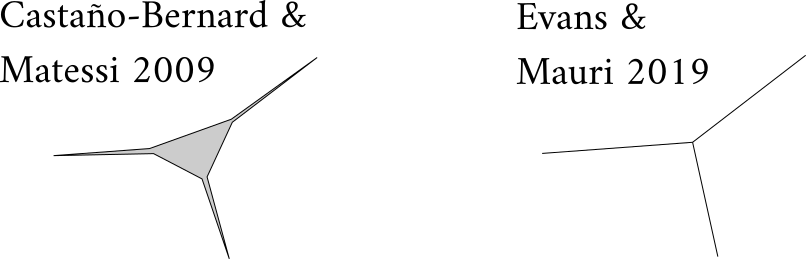
\includegraphics[width=200pt]{theorems}


\end{center}
\end{overprint}
\end{frame}
\begin{frame}
{Proof}
\begin{center}
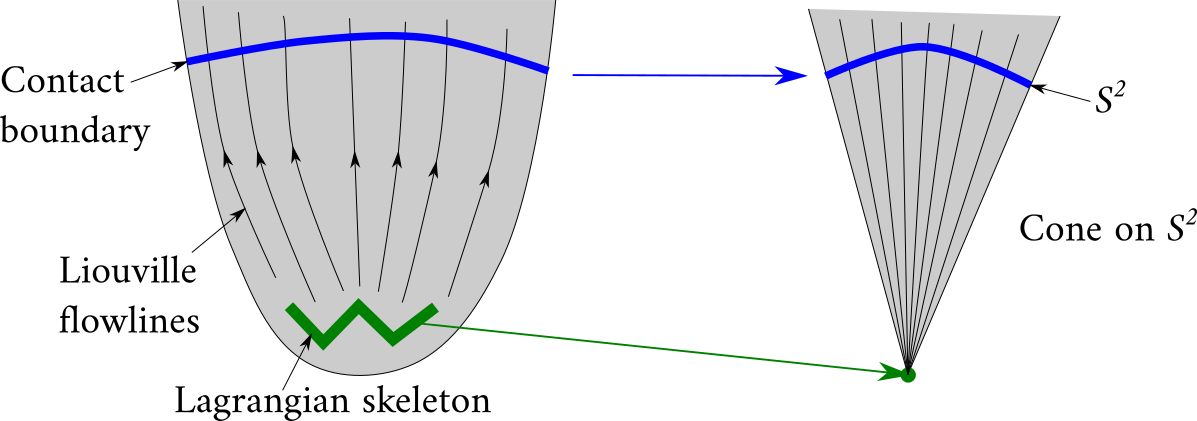
\includegraphics[width=310pt]{proof1}


\vspace{1cm}


\begin{minipage}[0.2\textheight]{\textwidth}
\begin{columns}[T]
\begin{column}{0.6\textwidth}
\begin{enumerate}
\item <2-> Lagrangian skeleton is Gross fibre.
\item <3> Contact boundary has LTF with three nodal fibres.
\end{enumerate}
\end{column}
\begin{column}{0.4\textwidth}
\begin{overprint}
\onslide<2>\centering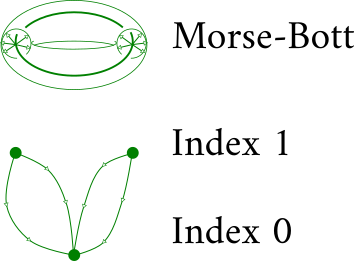
\includegraphics[width=100pt]{skeleton}
\onslide<3>\centering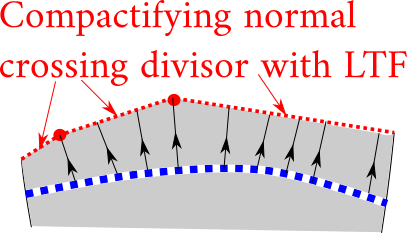
\includegraphics[width=100pt]{divisor}
\end{overprint}
\end{column}
\end{columns}
\end{minipage}
\end{center}
\end{frame}
\end{document}
